%% ------------- English version ---------------
\documentclass[english,hidelinks]{sbrt}
\usepackage{newtxtext}
\usepackage[english]{babel}
\usepackage[utf8]{inputenc}
\newtheorem{theorem}{Theorem}
%% ---------------------------------------------
\setlength{\marginparwidth}{2cm}
\usepackage{todonotes}
\newcommand\rigel[1]{\todo[color=green, inline]{\textbf{Rigel}: #1}}
\usepackage{orcidlink}
\usepackage{graphicx}
\usepackage{hyperref}
\usepackage[
  compatibility=false,
  font=footnotesize,
  labelsep=period,
  format=plain,
  justification=raggedright,
  singlelinecheck=false
]{caption}

\begin{document}

\title{Embedded Systems-based Predictive Maintenance for Air-Conditioning Equipment}

\author{Igor Costa, Jorge Alves, Ian Dias and Davi Ito
  \thanks{The authors are with Ibmec, Rio de Janeiro, RJ, Brazil.
  E-mails: igorcosta.silva10a@gmail.com,
  jorgedocruzeiro07@gmail.com,
  iandpcarvalho@gmail.com,
  cdavi8249@gmail.com.}%
  }

\maketitle

\markboth{XLIV BRAZILIAN SYMPOSIUM ON TELECOMMUNICATIONS AND SIGNAL PROCESSING - SBrT 2026, SEPTEMBER 29TH TO OCTOBER 2ND, 2026, SALVADOR, BA}{}

\begin{abstract}
Air-conditioning units run around the clock and rarely have a labelled failure history. This paper presents a low-cost embedded system that monitors their vibration and an open method that learns the healthy behavior of each unit where it is installed. An ESP32 reduces 1.24~s windows of a MEMS accelerometer to features, and a detector trained once compares each window with healthy windows of similar room climate. On a bench fan, it raised no false alarm in healthy tests and caught three real faults, unbalance, a loose part, and an obstruction, while a fixed limit caught only the unbalance.
\end{abstract}
\begin{keywords}
Predictive maintenance, air-conditioning systems, embedded systems, Internet of Things, anomaly detection.
\end{keywords}

\section{Introduction}

Air-conditioning units in hospital wards, data centers, and telecommunication shelters run around the clock, and their cooling cannot stop for inspection. Embedded Internet of Things (IoT) devices can watch such equipment continuously, acquiring measurements at the asset and processing them nearby \cite{gubbi2013iot}, so that maintenance acts before a failure. For HVAC systems, Es-Sakali et al. group the predictive approaches into knowledge-, physics-, and data-driven ones, the last built on the history of each system \cite{essakali2022hvac}.

\textit{Related work.} Yousuf et al. monitor induction motors with temperature, vibration, current, voltage, and speed sensors and alert when a user-set limit is crossed, and Mohammed et al. induce faults on one motor, such as an unbalance mass, and train classifiers on the labelled recordings, with Random Forest the most accurate \cite{yousuf2024iot,mohammed2023iot}. Kolok et al. compute RMS and FFT features on an ESP32 and train an Isolation Forest on healthy data from one controlled session, testing it on a wheel blocked on purpose \cite{kolok2025lowcost}, and Aung et al. run a classifier on an embedded board that reads an accelerometer on a fan, trained on labelled states of that fan \cite{aung2024fan}. Tormos et al. learn a baseline of bus air-conditioning units without fault labels, restricting it to one bus model, one route, and the hot hours of the day, and attribute each deviation to the variables that produced it \cite{tormos2026hvacxai}. Gupta et al. separate loaded from idle conveyor data before training and pool identical conveyors of one airport \cite{gupta2023baggage}. All of them train and test on the same machine or on identical machines under controlled conditions, and none moves a trained model to another installation \cite{meitz2025pdmframework}. Michau and Fink show that a detector trained on one unit misjudges conditions seen only on other units, and align units with adversarial deep learning, which needs the data of every unit \cite{michau2021transfer}.

This work asks whether one trained model can serve every unit and answers with measurements: it cannot, unless its margin is so wide that only severe faults show. What generalizes is the method. Our contribution is an open pipeline, from firmware to a training and checking tool, that learns the healthy behavior of each unit where it is installed, compares each window with the healthy windows of the most similar room climate, and names the measurement behind each alarm. On a fan fixed to a base, as a unit is installed, we record three real faults, an unbalanced blade, a loose part, and a blocked outlet, and show that each leaves its own mark. We also report the methods we discarded and why. A bench fan is not a compressor, so the results characterize the method rather than validate it on a real unit. Code, data, and documentation are public \cite{repo}.

\section{System Description}
\label{sec:system-description}

The prototype runs on a bench built around a 12~V fan, the same class of machine as the condenser fan of an air conditioner. The fan stands upright, glued with silicone to a wooden board, as a unit is fixed where it is installed. An ESP32 reads an ADXL345 MEMS accelerometer bonded to the fan frame, an INA219 shunt monitor in series with the supply, and a DHT11 for room temperature and humidity (Fig.~\ref{fig:architecture}). The accelerometer fills its FIFO at a measured 414~Hz, and the ESP32 forms windows of 512 samples, 1.24~s and 0.81~Hz of resolution. For each axis it computes RMS, peak, and kurtosis, and a Hann-windowed FFT gives the dominant frequency and its amplitude; the rotation of the fan, 46~Hz, appears as that frequency. The current is averaged over the window. The fan tachometer was dropped, since its loose wire read from 0 to 4900~rpm for the same motor. Each window leaves the board as one line of comma-separated fields over USB, since the campus network admits a device only after a web login; in the field, the board would publish over MQTT \cite{mohammed2023iot}. On a real unit, a split-core current transformer would replace the shunt and the accelerometer would be held to the compressor shell.

A recorder, a trainer, and a checker run on Windows or macOS without a network. The trainer takes the healthy recordings of a unit and stores its model in seconds, and the checker marks the windows of any recording that leave that model's normal.

\begin{figure}[t]
  \centering
  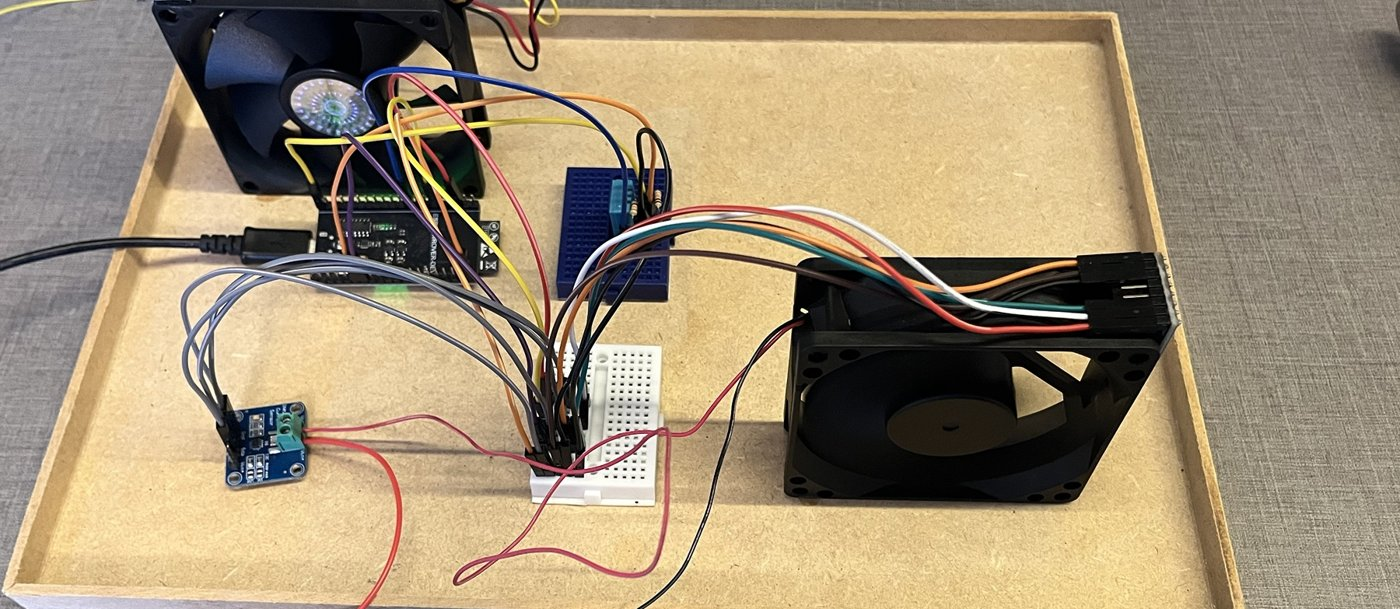
\includegraphics[width=0.92\columnwidth]{assets/bench-board-photo.jpg}\\[1pt]
  {\footnotesize (a) The bench.}\\[7pt]
  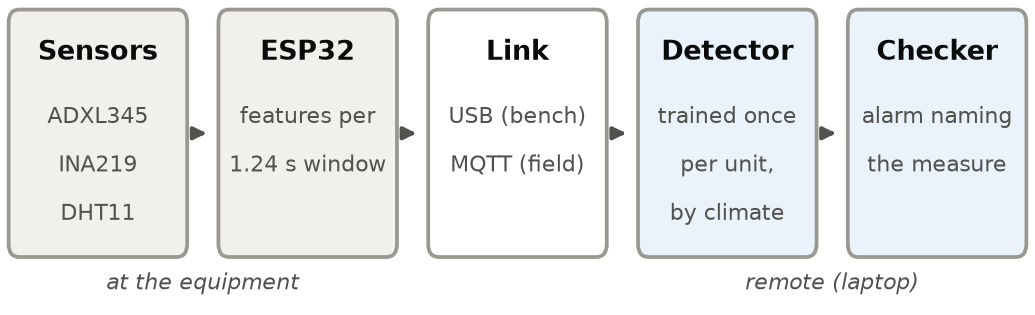
\includegraphics[width=\columnwidth]{assets/architecture-board.png}\\[1pt]
  {\footnotesize (b) The architecture.}
  \caption{The prototype. The monitored fan stands on the right with the ADXL345 on its top edge; the INA219, the ESP32, and the DHT11 sit on the same board. The fan at the back is not used.}
  \label{fig:architecture}
\end{figure}

\section{The Method}
\label{sec:method}

The detector watches five vibration totals per window that do not depend on the orientation of the sensor: the vector sums of RMS, peak, and spectral peak amplitude, the mean kurtosis, and the median dominant frequency. The current is recorded but raises no alarm: on the same board and with no fault it went from 154 to 142~mA between two days, following external factors such as the supply rather than the fan, and none of the recorded faults moved it. The detector is trained once, after maintenance, on healthy recordings, and never relearns, so wear that develops slowly stays visible. The room climate raises no alarm of its own; it selects the healthy windows that define normal. For each window, the normal is the median and spread of the 600 training windows, about 12 minutes, whose temperature and humidity are closest, with 1~$^\circ$C weighing as much as 5 points of humidity. The spread is $s=\max(1.4826\,\mathrm{MAD},\,0.03\,\tilde{x})$ around the median $\tilde{x}$, so a few shocks do not shift it.

Three tests run on every window, and any one raises an alarm. The ruler flags an RMS, peak, or spectral amplitude more than six spreads above normal and catches abrupt faults; these strengths count only when they rise, since a fan that vibrates less is not failing. An Isolation Forest of 200 trees, the detector of Kolok et al. and Tormos et al. \cite{kolok2025lowcost,tormos2026hvacxai}, judges whether the combination of the five deviations is unusual and counts only on two consecutive windows with some deviation of three spreads or more. The slow test takes the median of the last three minutes of the energy and the dominant frequency, leaving out the warm-up and the sway of the base below 10~Hz, and flags it when it leaves the range seen in training, which catches a fault too small for any single window. The first five minutes of every run are the motor warming up, when the vibration rose from 0.043 to 0.067~g, so they stay out of training and raise no alarm. Each alarm names the measurement that moved the most.

\textit{Methods tried.} The first detector, an Isolation Forest trained once on two healthy sessions as in Kolok et al., flagged 100\% of a third healthy session: the loose fan vibrated at 0.15~g on one table and 0.10~g on another, more than an obstruction changes it. The second, presented in the previous stage, relearned its baseline every minute and raised no false alarm, but it absorbs a fault that grows slowly, and clogging filters and wearing bearings grow slowly. The third, this detector trained in one place, caught a slow fault at 6 to 8\% above normal but flagged the whole of any other place, and pooling places removed those alarms at the cost of sensitivity. Fixing the fan to a board, as a unit is installed, brought the normal of five places within 0.057 to 0.066~g, against 0.10 to 0.18~g loose. On the board, a ruler in both directions flagged a fan that only vibrated less in a hotter room, and the current flagged a whole healthy day, which led to the present design.

\section{Results}
\label{sec:results}

The fan on its board was recorded healthy for 6.4~h on 11 and 12 November: five places of 5 to 30~min, a session of 14~min, a night of 4.5~h on a wooden bench at 26~$^\circ$C, and an afternoon of 53~min on the same bench at 30~$^\circ$C. After warm-up, the five places stayed within 0.057 and 0.066~g and the night within 0.065 and 0.068~g; in the warmer afternoon the fan vibrated 9\% less, at 0.060~g. The dominant frequency stayed at the rotation, 46~Hz, except for a sway of the board at 3 to 5~Hz in about one window in seven.

\textit{Real faults.} Three faults were made on the same bench (Fig.~\ref{fig:faults}). A thumb-sized piece of tape glued firmly to the middle of one blade unbalanced the rotor: the vibration rose 55\%, to 0.103~g, with the frequency still at 46~Hz. The same tape glued loosely flapped and could be heard: the vibration stayed near normal but became irregular, and the dominant frequency doubled to 93~Hz. A heavy wooden block 2 to 5~cm from the outlet left the vibration at normal and dropped the dominant frequency to 15~Hz, about a third of the rotation, as in rotating stall when the air has nowhere to go; in the same heat without the block it stayed at 46~Hz. When the firm tape later began to come off, the vibration reached 0.20~g within two minutes before the tape flew away.

\begin{figure*}[t]
  \centering
  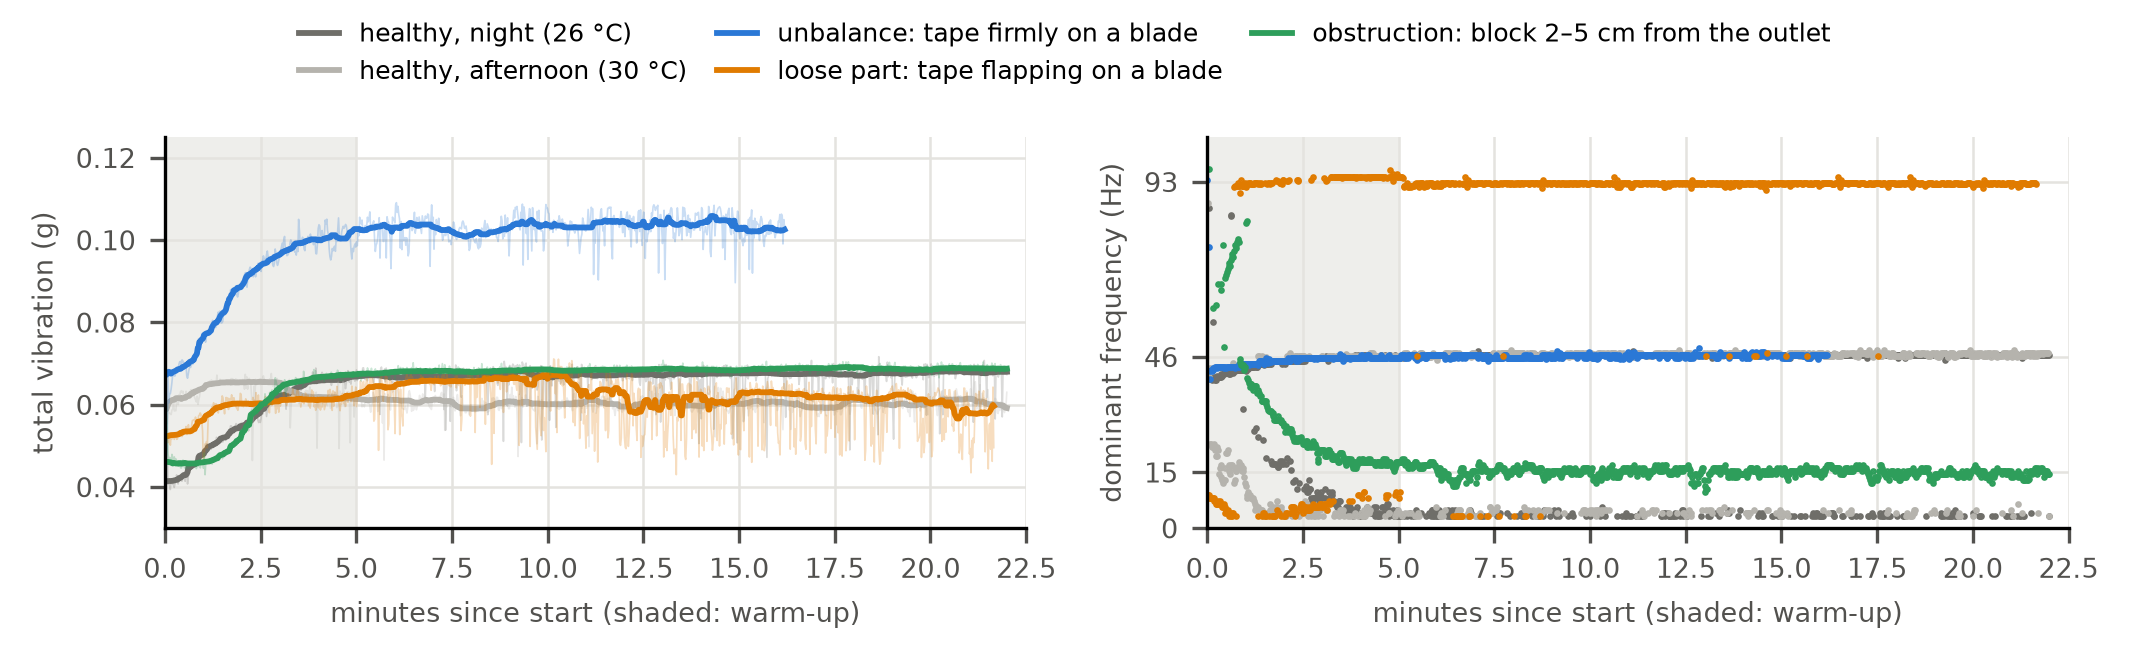
\includegraphics[width=\textwidth]{results/real_faults.png}
  \caption{Total vibration (median of 45 windows over each window) and dominant frequency of the fan fixed to its board, healthy and with three real faults on the same bench. Unbalance raises the vibration; a loose part doubles the dominant frequency; an obstruction drops it.}
  \label{fig:faults}
\end{figure*}

\begin{table}[t]
\caption{False alarms on healthy test segments, and windows in alarm and delay to a steady alarm for each real fault appended after healthy operation.}
\label{tab:results}
\centering
\setlength{\tabcolsep}{4pt}
\begin{tabular}{lccc}
\hline
 & Trained & Adaptive & Fixed limit \\
\hline
False alarm, night & 0.0\% & 7.8\% & 0.0\% \\
False alarm, afternoon & 0.0\% & 0.1\% & 0.0\% \\
False alarm, 11 Nov. & 0.0\% & 5.1\% & 0.0\% \\
Unbalance & 100\%, 0 min & 100\%, 0 min & 100\%, 0 min \\
Loose part & 92\%, 1 min & 19\%, 17 min & never \\
Obstruction & 100\%, 0 min & 100\%, 0 min & never \\
Slow fault, night & +8\% & never & +25\% \\
\hline
\end{tabular}
\end{table}

\textit{Comparison.} The detector was trained on the first 200~min of the night and the first 28~min of the afternoon, and tested on the rest. Each fault was recorded from start-up, so for testing it was appended after a healthy segment, as a fault appears in service. Table~\ref{tab:results} compares it with the adaptive detector and with a fixed limit at 1.25 times the median vibration of training. The trained detector raised no false alarm and caught the three faults, the loose part within a minute. The fixed limit saw only the unbalance, the one fault that raises the vibration. The adaptive detector raised 5 to 8\% of false alarms and saw the loose part late; started on a fan that already had the tape, it learned the unbalance as normal and flagged the whole healthy run after the tape flew away. For a simulated slow fault of 1\% per minute, the trained detector alarmed at 8\% above normal at night and 4\% in the afternoon; the fixed limit alarmed at 25\% at night and never in the shorter afternoon, and the adaptive detector never, since it learns a slow fault as normal. Each fault was made once on one fan, so these results show how each fault appears more than how often it is caught.

\section{Conclusion}
\label{sec:conclusion}

A detector trained once catches slow faults that an adaptive one learns as normal and that a fixed limit sees late, and on a fan fixed to its base it caught three real faults, each through a different measurement: the unbalance through the vibration, the loose part and the obstruction through the dominant frequency, which no limit on the vibration sees. Its normal holds only where it was learned: the loose fan looked faulty in a new place, and the fan on its board vibrated less in a warmer room, so one model for every air conditioner would need a margin so wide that only severe faults show. What generalizes is the method, published as an open pipeline in which each unit learns its own normal, with its room climate, where it is installed. The results have clear limits: each fault was made once on one fan, the climate spanned 26 to 30~$^\circ$C, the recordings cover hours rather than months, and a bench fan is not a compressor, whose current, here moved only by external factors, should follow its load. The next steps are repeating each fault in other climates and days, measuring how many minutes of training suffice and how stable the normal stays across days, and testing the method on a real unit.

\bibliographystyle{ieeetr}
\bibliography{refs}

\end{document}
